%%%%%%%%%%%%%%%%%%%%%%%%%%%%%%%%%%%%%%%%%%%%%%%%%%%%%%%%%%%%%%%%%%%%%%%%%%%%%%%%
%2345678901234567890123456789012345678901234567890123456789012345678901234567890
%        1         2         3         4         5         6         7         8

\documentclass[letterpaper, 10 pt, conference]{ieeeconf}  % Comment this line out if you need a4paper
\usepackage{amsmath, xparse}
\usepackage{amstext}
\usepackage{amsfonts}
\usepackage{float}
\usepackage{graphicx}
\usepackage{hyperref}
\usepackage[utf8]{inputenc}
\usepackage{algorithm}
\usepackage[noend]{algpseudocode}
\usepackage{caption}

\usepackage{adjustbox}
\usepackage{booktabs}

\usepackage{outlines}


\makeatletter
\renewcommand{\Function}[2]{%
  \csname ALG@cmd@\ALG@L @Function\endcsname{#1}{#2}%
  \def\jayden@currentfunction{#1}%
}
\newcommand{\funclabel}[1]{%
  \@bsphack
  \protected@write\@auxout{}{%
    \string\newlabel{#1}{{\jayden@currentfunction}{\thepage}}%
  }%
  \@esphack
}
\makeatother

%\documentclass[a4paper, 10pt, conference]{ieeeconf}      % Use this line for a4 paper

\IEEEoverridecommandlockouts                              % This command is only needed if
                                                          % you want to use the \thanks command

\overrideIEEEmargins                                      % Needed to meet printer requirements.

%In case you encounter the following error:
%Error 1010 The PDF file may be corrupt (unable to open PDF file) OR
%Error 1000 An error occurred while parsing a contents stream. Unable to analyze the PDF file.
%This is a known problem with pdfLaTeX conversion filter. The file cannot be opened with acrobat reader
%Please use one of the alternatives below to circumvent this error by uncommenting one or the other
%\pdfobjcompresslevel=0
%\pdfminorversion=4

% See the \addtolength command later in the file to balance the column lengths
% on the last page of the document

% The following packages can be found on http:\\www.ctan.org
%\usepackage{graphics} % for pdf, bitmapped graphics files
%\usepackage{epsfig} % for postscript graphics files
%\usepackage{mathptmx} % assumes new font selection scheme installed
%\usepackage{times} % assumes new font selection scheme installed
%\usepackage{amsmath} % assumes amsmath package installed
%\usepackage{amssymb}  % assumes amsmath package installed

\title{\LARGE \bf
Final Report: \\ 
\Large AlienGLRenderer Cloth Simulation
}



\author{Arrian Chi% <-this % stops a space
\\
\\
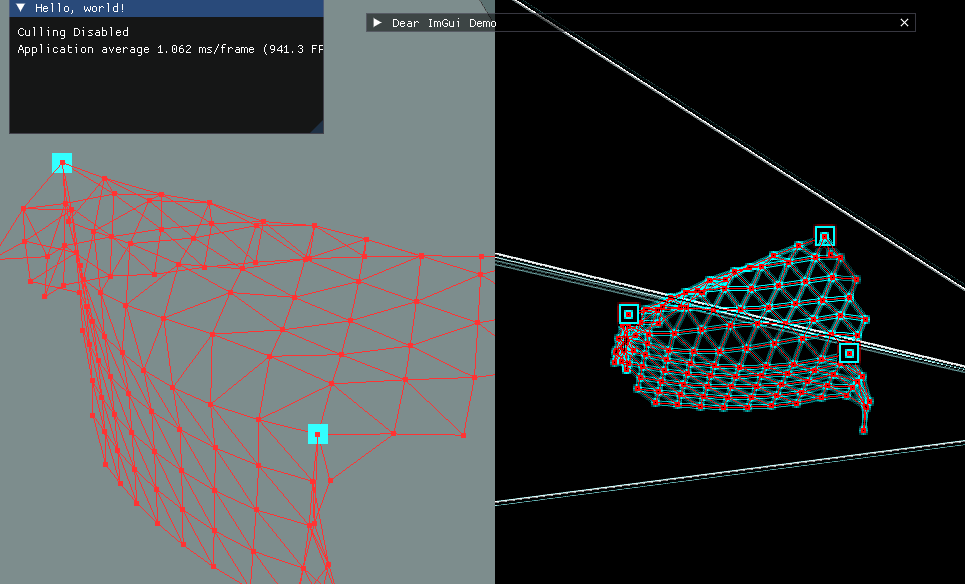
\includegraphics[width=8cm]{cloth1.PNG} \> 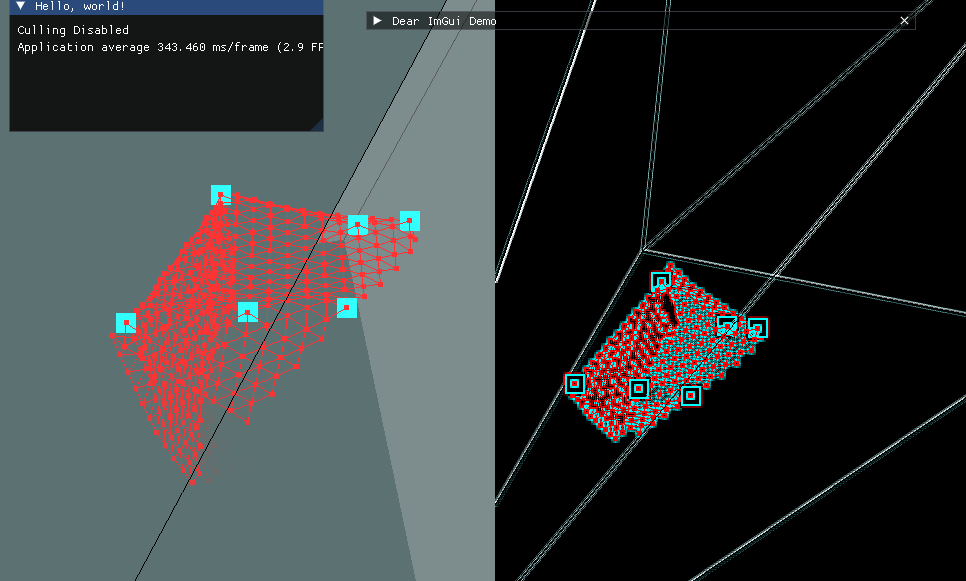
\includegraphics[width=8cm]{cloth2.PNG} 
}




\begin{document}

% \onecolumn


\maketitle
\thispagestyle{empty}
\pagestyle{empty}


%%%%%%%%%%%%%%%%%%%%%%%%%%%%%%%%%%%%%%%%%%%%%%%%%%%%%%%%%%%%%%%%%%%%%%%%%%%%%%%%

\begin{abstract}

Cloth simulations have been a staple problem in computer graphics for a long time. They are used in movies, video games, and even in scientific simulations. The DEP/S algorithm is a popular algorithm used to simulate cloth in real-time. In this project, I implemented the DEP/S algorithm in C++ using the Eigen library and OpenGL. This report talks about the intricacies and details that come into play when implementing a cloth simulation. 

\end{abstract}
\section{Overview}

Research in computer graphics from the past few decades to the present \cite{baraff1998large} \cite{Grinspun2003discrete} \cite{Tamstorf2013discrete} has shown particular interest in the simulation of plates, cloth, and other thin materials. These simulations are used in movies, video games, and even in scientific simulation. Various algorithms have been developed to simulate these materials, such as geometric approximations from cable theory \cite{weil1986synthesis}, more physically involved methods simulating the cloth as a connected mass-spring damper system  \cite{provot1995deformation}, and even more physically accurate models con sidering the elastic energies within the discretized simulated cloth \cite{terzopoulos1987elastically}. 

A realization of the last point is the well-known Discrete Elastic Plates / Shells numerical simulation algorithm, shown in Algorithm 1 \cite{jawedlimdiscrete} \cite{baraff1998large}. To explain, the algorithm discretizes the cloth into particle masses arranged in a mesh. In the simulation loop, where each iteration represents a step in time (thus a change in cloth position), it calculates the forces acting upon the particles to find what the next positions of the particles will be. The algorithm specifically uses the Newton-Raphson method to solve for the positions of the particles, so calculating and solving for the gradient (forces) and Hessians(Jacobian of forces) of elastic energies within the cloth is a necessary step. The elastic energies occur as stretching energies, along the edges between each particle, and bending energies at every edge adjacent to two faces of the mesh. An error is calculated at the end of the method to determine if the calculation has converged, and if not, the simulation continues to iterate until the error is less than a certain tolerance. Once the new position is obtained, the simulation continues to the next time step.

% \begin{figure*}[p]
%         \centering

% \label{"fig:dep"}

For this project, I wanted to integrate a feature into my hobby renderer, AlienGLRenderer. The renderer's main purpose is to serve as a sandbox for me to implement and showcase graphics features I am interested in the moment and to improve my skills in C++. Thus, I decided to  implement cloth simulation feature using the DEP/S algorithm in it. Because my renderer is akin to a game engine, I made it my goal to make the cloth update and render in real-time with OpenGL and C++. A link to the project source can be found here: \url{https://github.com/dinoplane/gl_alien_renderer/tree/cloth-system}.

In my initial proposal, I posed a few questions I would like my project to answer. Through the course of the project, these questions have drastically changed, so to update, these questions now are:
\begin{outline}[enumerate]
        \1 How efficient can a cloth simulation be?
        \1 How do we simulate a cloth efficiently?
                \2 Where could the DEP algorithm benefit from optimization?
                        \3 What parameters affect the efficiency of the algorithm?
                \2 Is multi-threading useful or not?
                \2 Could we afford a tradeoff between stability and speed? 
                \2 What is the source of instability?
        \1 What technical problems/constraints arise when simulating cloth?
                \2 Are there technical complexities during development that were frustrating?
\end{outline}


\onecolumn
        \begin{algorithm}[h]
                \caption{Discrete Elastic Plates}
                \textbf{Require:} $q(t_{i}), \dot{q}(t_{i})$ \hfill \texttt{DOFs and velocities at } $t_i$\\
                \hspace*{10mm} $e(m), h(n)$ \hfill \texttt{m edges and n hinges present in the plate}\\
                \hspace*{10mm} $m, M$ \hfill \texttt{masses of each particle (as a vector and matrix)}\\ 
                \hspace*{10mm} $l_{k}, k_{s}$ \hfill \texttt{undeformed length / stretching  for each edge}\\
                \hspace*{10mm} $\bar{\theta}, k_b$ \hfill \texttt{rest angles of each hinge, bending stiffness} \\                
                \hspace*{10mm} $\Delta t$ \hfill \texttt{time step}\\
                \hspace*{10mm} $\mathbf{f^{ext}}$ \hfill \texttt{external forces}\\ 
                \hspace*{10mm} \texttt{free\_index} \hfill \texttt{Index of the free DOFs}\\ \\
                \textbf{Ensure:} $q(t_{i+1}), \dot{q}(t_{i+1})$ \hfill \texttt{DOFs and velocities at } $t = t_{i+1}$\\

                \begin{algorithmic}[1]
                        \Function{Compute\_Stretching}{$q, e, l_{k}, k_{s}$}
                                \State $\mathbf{f^{stretch}},\mathbf{J^{stretch}}  \gets 0, 0$ \hfill \texttt{Initialize}
                                \For{$i \gets 1$ to $m$}
                                        \State \texttt{x0}, \texttt{x1} $\gets q(e(k, 1)), \, q(e(k, 2))$ \hfill \texttt{Get DOFs of particles in edges}
                                        \State $\mathbf{f^{grad}}, \mathbf{J^{hess}} \gets \Call{GradEs\_HessEs}{\texttt{x0}, \texttt{x1}, l_{k}(i), k_{s}(i)}$ \hfill Refer to Appendix of \cite{jawedlimdiscrete} \\
                                        \State $\mathbf{f^{stretch}}(e(k)) \gets \mathbf{f^{stretch}}(e(k)) - \mathbf{f^{grad}}$ \hfill \texttt{Update total force/Jacobian}
                                        \State $\mathbf{J^{stretch}}(e(k), e(k)) \gets \mathbf{J^{stretch}}(e(k), e(k)) - \mathbf{J^{hess}}$
                                \EndFor
                                \State \Return $\mathbf{f^{stretch}}, \mathbf{J^{stretch}}$
                        \EndFunction \\ 
                
                        \Function{Compute\_Bending}{$q, h, k_b$}
                                \State $\mathbf{f^{bend}},\mathbf{J^{bend}}  \gets 0, 0$ \hfill \texttt{Initialize}
                                \For{$i \gets 1$ to $n$}
                                        \State \texttt{x0}, \texttt{x1}, \texttt{x2}, \texttt{x3} $\gets q(e(k, 1)), \,  q(e(k, 2)), \, q(e(k, 3)), \, q(e(k, 4))$ \hfill \texttt{Get DOFs of particles in hinges}
                                        \State $\mathbf{f^{grad}}, \mathbf{J^{hess}} \gets \Call{GradEb\_HessEb}{\texttt{x0}, \texttt{x1}, \texttt{x2}, \texttt{x3}, l_{k}(i), k_{s}(i)}$ \hfill Refer to Appendix of \cite{jawedlimdiscrete} \\
                                        \State $\mathbf{f^{bend}}(e(k)) \gets \mathbf{f^{bend}}(e(k)) - \mathbf{f^{grad}}$ \hfill \texttt{Update total force/Jacobian}
                                        \State $\mathbf{J^{bend}}(e(k), e(k)) \gets \mathbf{J^{bend}}(e(k), e(k)) - \mathbf{J^{hess}}$
                                \EndFor
                                \State \Return $\mathbf{f^{bend}}, \mathbf{J^{bend}}$
                        \EndFunction \\
                
                \Function{Discrete\_Elastic\_Plates}{$q, \dot{q}$} 
                    \State Guess: $q^{(1)}(t_{i+1}) \gets q(t_i)$
                    \State $n \gets 1$
                    \While{$\text{error} > \text{tolerance}$} \\
                        \State $\mathbf{f^{stretch}}, \mathbf{J^{stretch}}  \gets \Call{Compute\_Stretching}{q, e, l_{k}, k_{s}}$ 

                        \State $\mathbf{f^{bend}}, \mathbf{J^{bend}}  \gets \Call{Compute\_Bending}{q, e, l_{k}, k_{s}}$ \\
                                
                        \State $\mathbf{f^{tot}} \gets \mathbf{f^{bend}} + \mathbf{f^{stretch}} + \mathbf{f^{ext}}$ \hfill \texttt{Aggregate forces}
                        \State $\mathbf{f} \gets \frac{1}{\Delta t}m \odot \left[\frac{1}{\Delta t} \left[q^{(n)} - q^{(1)}\right] - \dot{q} \right] - \mathbf{f^{tot}}$ \\

                        \State $\mathbf{J^{tot}} \gets \mathbf{J^{bend}} + \mathbf{J^{stretch}}$ \hfill \texttt{Aggregate Jacobians}
                        \State $\mathbf{J} \gets \frac{1}{\Delta t} M - \mathbf{J^{tot}}$ \\
                        
                        \State $\mathbf{f}_\text{free} \gets \mathbf{f}(\texttt{free\_index})$
                        \State $\mathbf{J}_\text{free} \gets \mathbf{J}(\texttt{free\_index}, \texttt{free\_index})$\\
                        \State $\Delta q_\text{free} \gets \mathbf{J}_\text{free}^{-1} \mathbf{f}_\text{free}$
                        \State $q^{(n+1)}(\texttt{free\_index}) \gets q^{(n)}(\texttt{free\_index}) - \Delta q_\text{free}$ \hfill \texttt{Update free DOFs}
                        \State $\text{error} \gets \text{sum}(\lvert \mathbf{f}_\text{free} \rvert)$
                        \State $n \gets n + 1$ \\
                    \EndWhile
                    \State $q(t_{i+1}) \gets q^{(n)}(t_{i+1})$                  \hfill \texttt{Update DOFs for next time step}
                    \State $\dot{q}(t_{i+1}) \gets \dot{q}^{(n)}(t_{i+1})$
                \EndFunction
                \end{algorithmic}
                \end{algorithm}
        % \end{figure*}
\twocolumn


This is a lot of questions, so I will organize the report into 3 sections: Results, Process, and Issues. 

\section{Results}
I tested my simulation on an AMD Ryzen 9 7900 (with integrated graphics). The configuration of the mesh was akin to that of a table cloth (see figure \ref{fig}) There are three iterations of my simulation: a dense matrix version, a sparse matrix version, and PARDISO solver version. A table of the data collected can be seen in figures \ref{}. The data is displayed on a graph in figures \ref{"fig:"}. As one can see, each version's frame times are vary widely, each incurring improvement over the next. 

Using the dense matrix version as a base, the sparse matrix incurred an $8\times$ speedup and the PARDISO solver version incurred a $10\times$ max speedup. These speedups are drastic and just goes to show how much dense matrices can be a bottleneck in the simulation. Comparing the sparse matrix version to the PARDISO solver version, the PARDISO solver version is at least $1.3\times$ faster than the sparse matrix version. This is expected since the PARDISO solver is more specialized towards solving the symmetric sparse matrices that the DEP algorithm produces.

The graphs also tell a telling story, the dense matrix version frame time grows consistently with the predicted $O(n^3)$ time complexity (mostly from the matrix solve), breaking 800ms per frame at 529 nodes. The sparse matrix and PARDISO solver versions grow at a much flatter linear-like rate, with the PARDISO solver breaking 81ms per frame at 529 nodes compared to the sparse matrix version's 87ms per frame.

Finally, it is worth mentioning that the ratio between the force calculation time and the solver time was consistently less than 1 after 81 nodes. This further proves that the solver is the bottleneck of the simulation in that version. On both the sparse matrix and PARDISO solver versions, the ratio rose and fell. This suggests that starting with a small number of nodes, the solver produced enough overhead that made it slower than the force calculation, but as the number of nodes increased, the force calculation became the bottleneck. This would not last long when the number of nodes increases even further, we are introduced to the solver bottleneck again.

\onecolumn
\begin{figure}
\begin{minipage}[b]{.45\linewidth}
                \centering
                \begin{tabular}{|c|c|c|c|c|}
                \hline
                \textbf{Side Length} & \textbf{\# Nodes} & \textbf{\# DOFs} & \textbf{\#Edge} & \textbf{\# Hinge} \\ \hline
                1                    & 4                    & 12                  & 5                   & 1                    \\ \hline
                2                    & 9                    & 27                  & 16                  & 8                    \\ \hline
                3                    & 16                   & 48                  & 33                  & 21                   \\ \hline
                4                    & 25                   & 75                  & 56                  & 40                   \\ \hline
                5                    & 36                   & 108                 & 85                  & 65                   \\ \hline
                6                    & 49                   & 147                 & 120                 & 96                   \\ \hline
                7                    & 64                   & 192                 & 161                 & 133                  \\ \hline
                8                    & 81                   & 243                 & 208                 & 176                  \\ \hline
                9                    & 100                  & 300                 & 261                 & 225                  \\ \hline
                10                   & 121                  & 363                 & 320                 & 280                  \\ \hline
                11                   & 144                  & 432                 & 385                 & 341                  \\ \hline
                12                   & 169                  & 507                 & 456                 & 408                  \\ \hline
                13                   & 196                  & 588                 & 533                 & 481                  \\ \hline
                14                   & 225                  & 675                 & 616                 & 560                  \\ \hline
                15                   & 256                  & 768                 & 705                 & 645                  \\ \hline
                16                   & 289                  & 867                 & 800                 & 736                  \\ \hline
                17                   & 324                  & 972                 & 901                 & 833                  \\ \hline
                18                   & 361                  & 1083                & 1008                & 936                  \\ \hline
                19                   & 400                  & 1200                & 1121                & 1045                 \\ \hline
                20                   & 441                  & 1323                & 1240                & 1160                 \\ \hline
                21                   & 484                  & 1440                & 1365                & 1281                 \\ \hline
                22                   & 529                  & 1575                & 1496                & 1408                 \\ \hline
                \end{tabular}
                \caption{A table of plate properties per side length \#} \label{fig:plateproperties} 
        \end{minipage} \\


        \begin{minipage}[b]{.45\linewidth}
                \begin{center}
                        \begin{tabular}{|c|c|c|c|}
                        \hline
                        \textbf{\# Nodes} & \textbf{Dense} & \textbf{Sparse} & \textbf{PARDISO} \\ \hline
                        4                 & 2.14568        & 1.9417          & 1.97905          \\ \hline
                        9                 & 2.09046        & 1.86291         & 2.07927          \\ \hline
                        16                & 2.19543        & 1.87658         & 1.90431          \\ \hline
                        25                & 2.26691        & 1.9805          & 2.17057          \\ \hline
                        36                & 2.32498        & 2.02624         & 2.2378           \\ \hline
                        49                & 2.26632        & 2.17572         & 2.42311          \\ \hline
                        64                & 2.55798        & 2.38529         & 3.17389          \\ \hline
                        81                & 3.13174        & 3.07915         & 3.64856          \\ \hline
                        100               & 4.36049        & 3.40046         & 5.1266           \\ \hline
                        121               & 10.8998        & 5.11832         & 7.15082          \\ \hline
                        144               & 29.2132        & 5.81131         & 11.5085          \\ \hline
                        169               & 38.4439        & 14.5564         & 13.0989          \\ \hline
                        196               & 58.0018        & 23.1701         & 22.7056          \\ \hline
                        225               & 72.0361        & 27.0657         & 27.7778          \\ \hline
                        256               & 117.31         & 33.3114         & 32.7209          \\ \hline
                        289               & 133.053        & 44.3635         & 36.9456          \\ \hline
                        324               & 210.592        & 50.7165         & 39.6869          \\ \hline
                        361               & 266.549        & 66.6435         & 47.0635          \\ \hline
                        400               & 323.052        & 81.0222         & 60.7701          \\ \hline
                        441               & 574.367        & 84.1108         & 65.9397          \\ \hline
                        484               & 638.038        & 92.7115         & 74.1809          \\ \hline
                        529               & 873.053        & 105.039         & 81.0643          \\ \hline
                        \end{tabular}
                \end{center}
                \captionof{table}{A table of average frame times (ms/frame) per plate per simulation } \label{fig:frametimes}
        \end{minipage}\hfill
        \begin{minipage}[b]{.45\linewidth}
                \centering
                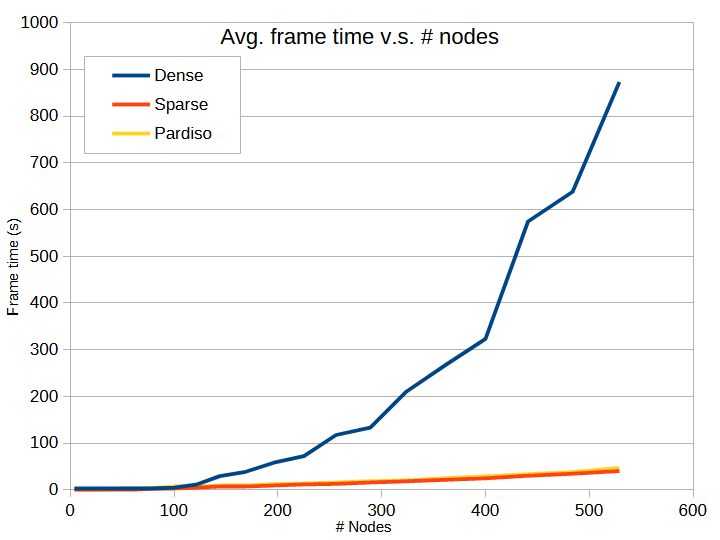
\includegraphics[width=1.1\linewidth]{frametimes.PNG}
                \captionof{figure}{Graph of average frame times per simulation}% \caption{Figure caption}
        \end{minipage}
\end{figure}

\begin{figure}
        \begin{minipage}[b]{.45\linewidth}
                \begin{center}
                        \begin{tabular}{|c|c|c|c|}
                        \hline
                        \textbf{\# Nodes} & \multicolumn{1}{c|}{\textbf{Dense}} & \multicolumn{1}{c|}{\textbf{Sparse}} & \multicolumn{1}{c|}{\textbf{PARDISO}} \\ \hline
                        4                 & 1.189                               & 1.178                                & 0.031                                 \\ \hline
                        9                 & 4.007                               & 0.328                                & 0.124                                 \\ \hline
                        16                & 3.856                               & 2.932                                & 0.323                                 \\ \hline
                        25                & 3.166                               & 1.867                                & 0.468                                 \\ \hline
                        36                & 2.496                               & 1.728                                & 0.649                                 \\ \hline
                        49                & 1.726                               & 1.521                                & 0.741                                 \\ \hline
                        64                & 1.294                               & 1.145                                & 0.862                                 \\ \hline
                        81                & 0.982                               & 1.223                                & 0.912                                 \\ \hline
                        100               & 0.689                               & 0.955                                & 0.880                                 \\ \hline
                        121               & 0.565                               & 0.895                                & 1.007                                 \\ \hline
                        144               & 0.448                               & 0.827                                & 1.131                                 \\ \hline
                        169               & 0.322                               & 0.891                                & 1.101                                 \\ \hline
                        196               & 0.298                               & 0.734                                & 1.118                                 \\ \hline
                        225               & 0.237                               & 0.969                                & 1.159                                 \\ \hline
                        256               & 0.189                               & 0.904                                & 1.179                                 \\ \hline
                        289               & 0.175                               & 0.627                                & 1.194                                 \\ \hline
                        324               & 0.143                               & 0.629                                & 1.115                                 \\ \hline
                        361               & 0.123                               & 0.544                                & 1.305                                 \\ \hline
                        400               & 0.110                               & 0.575                                & 1.210                                 \\ \hline
                        441               & 0.102                               & 0.703                                & 1.134                                 \\ \hline
                        484               & 0.085                               & 0.549                                & 1.140                                 \\ \hline
                        529               & 0.075                               & 0.513                                & 1.069                                 \\ \hline
                        \end{tabular}
        \end{center}
        \captionof{table}{A table of ratio of force calculation time to solver time} \label{fig:ratios}
        \end{minipage}\hfill
        \begin{minipage}[b]{.45\linewidth}
                \centering
                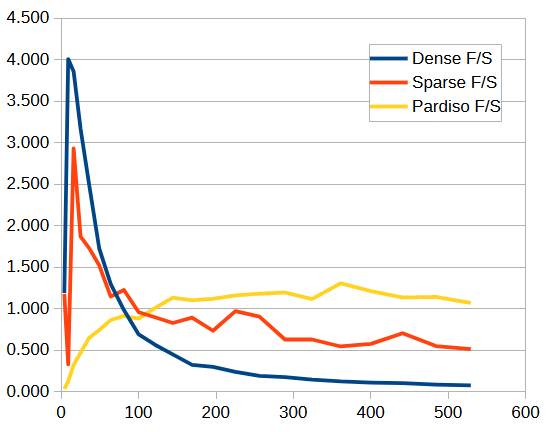
\includegraphics[width=1.1\linewidth]{ratios.png}
                \captionof{figure}{Graph of ratio of force to solver time}% \caption{Figure caption}
        \end{minipage}
\end{figure}

\begin{figure}
        \begin{minipage}[b]{.45\linewidth}
                \centering
                \begin{center}
                                \begin{tabular}{|c|c|c|c|} \hline
                                \textbf{\# Nodes} & D / S & D / P & S / P \\ \hline
                                64                & 1.072          & 0.806           & 0.752            \\ \hline 
                                81                & 1.017          & 0.858           & 0.844            \\ \hline
                                100               & 1.282          & 0.851           & 0.663            \\ \hline
                                121               & 2.130          & 1.524           & 0.716            \\ \hline
                                144               & 5.027          & 2.538           & 0.505            \\ \hline
                                169               & 2.641          & 2.935           & 1.111            \\ \hline
                                196               & 2.503          & 2.555           & 1.020            \\ \hline
                                225               & 2.662          & 2.593           & 0.974            \\ \hline
                                256               & 3.522          & 3.585           & 1.018            \\ \hline
                                289               & 2.999          & 3.601           & 1.201            \\ \hline
                                324               & 4.152          & 5.306           & 1.278            \\ \hline
                                361               & 4.000          & 5.664           & 1.416            \\ \hline
                                400               & 3.987          & 5.316           & 1.333            \\ \hline
                                441               & 6.829          & 8.710           & 1.276            \\ \hline
                                484               & 6.882          & 8.601           & 1.250            \\ \hline
                                529               & 8.312          & 10.770          & 1.296            \\ \hline
                                \end{tabular}
                \end{center}
                \captionof{table}{Simulation Speedups (D=Dense, S=Sparse, P=PARDISO)} 
                \label{fig:speedups}
        \end{minipage}\hfill
        \begin{minipage}[b]{.45\linewidth}
                \centering
                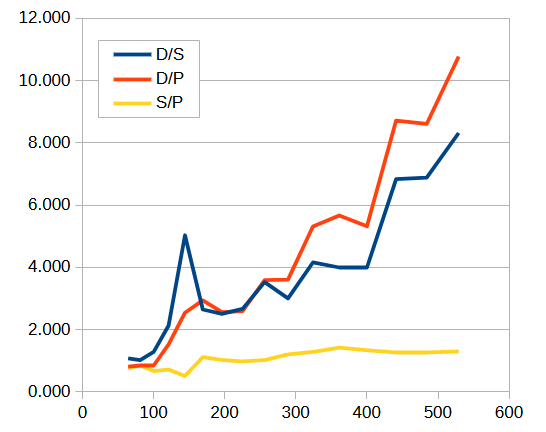
\includegraphics[width=1.1\linewidth]{speedups.png}
                \captionof{figure}{Graph of simulation speedups}% \caption{Figure caption}
        \end{minipage}
\end{figure}

\twocolumn

\section{Process}
 In the course of development for the cloth simulation, many amusing and interesting problems arose that I believe warrant discussion. In this section, I will provide a more in-depth explanantion of the implementation and highlight some key implementation details of the cloth simulation.

\subsection{Cloth Mesh Creation and Parameterization}
The mesh of the cloth is represented as a equilateral triangluar grid of particles connected by edges / hinges. The point positions are procedurally derived and dependent on a user supplied number of edges of the cloth and the edge length. In addition, the user also specifies the young's modulus, the thickness, the gravitational pull, and the timestep of the simulation.

\subsection{First iteration of the Discrete Elastic Plate / Shells Algorithm Implementation}

My implementation of the DEP Algorithm started out as a transcription of a python implementation that we went over during class. I leveraged the Eigen Library \cite{eigen_library} to handle the linear algebra computations in the algorithm. All calculations used the DenseMatrix object (which internally leverages a 2D array of numbers, a contiguous chunk of floats/doubles in memory). For the solver, I directly solved the matrix using the built in Eigen solver (LDLT solver). The outputs were verified by running the same input with the python implementation and comparing the results. This method of verification proved effective, since it revealed the first issue. 

My renderer defaulted to using float (single precision floating point numbers) for all of its calculations. That is a good decision because there was no need for precision in calculations and floats are only 4 bytes in size (the same as a int on most environments). However, upon closer inspection, the python implementation used double precision floats (8 bytes in size). This caused the results of the C++ implementation to be off by a small amount. The error was small enough that it was negligible for small values of n, but as n increased, the error accumulated and the results diverged. This was fixed by changing all the floats to doubles in the C++ implementation. Rendering still used floats, so I had to create a buffer that cast all the double values to floats before sending it to the GPU.

As shown in the results, the performance of initial simulation was abysmal. Both steps of the simulation, the force/Jacobian calculation and the solver, started staggering when the cloth side length was about 13-14 nodes (588-675 DOFs). At this stage, the solver took about 65\% of the total CPU time, while the force calculation took about 17\%. I believed that these steps can be optimized with multi-threading, but that proved to be slightly wrong. 

Eigen already allows users to enable multi-threading capabilities implemented for matrix arithmetic. However, for solving, it only supports multithreaded solves with sparse matrices (without additional extensions \cite{eigen_library}). In pursuit of this optimization, I changed the dense matrices involved in the calculation to use sparse matrices. As seen in the previous section, there was a speedup when this was implemented, which I will explain shortly. 

\subsection{Second iteration of the DEP/S Algorithm: Sparse Matrices and Multithreading}
Sparse matrices are matrices that have a large number of zero values compared to the number of nonzero values. If we used a dense matrix to represent a sparse matrix, there would be a whole lot of wasted space in memory. Additionally, when calculating arithmetic, sparse matrices would take a long time with no value because most of the arithmetic operations would end up being zero. 


To solve this issue, sparse matrix implementations usually involve only 3 arrays: One for the nonzero values, one for the row indices of the nonzero values in the matrix, and one for the indices(into the value array) of the first nonzero value in each row per column (see Fig \ref{fig:sparse_matrix}). This representation (also known as the Compressed Sparse Format) is much more compact, and because there are less elements to iterate through(skipping through all the zero values), the arithmetic operations and solving algorithms are faster. To create the sparse matrix, it is best to supply the constructor with an array of triplets (row, col, val) for each entry in the desired matrix. So I had to change the force calculations to append these elements to an existing array of triplets (a.k.a. sparse entries) for the Jacobian force matrix (the calculation of the hessians per edge/hinge are still done with fixed-size dense matrices). This method was fine since the bending jacobian and the stretching jacobian are added later in the algorithm and duplicate items in the sparse entry array are summed up. Using this scheme and changing the solver to use the Conjugate Gradient Iterative solver, I secured a 4x speedup (as seen in the above).

\begin{figure}
        \centering
        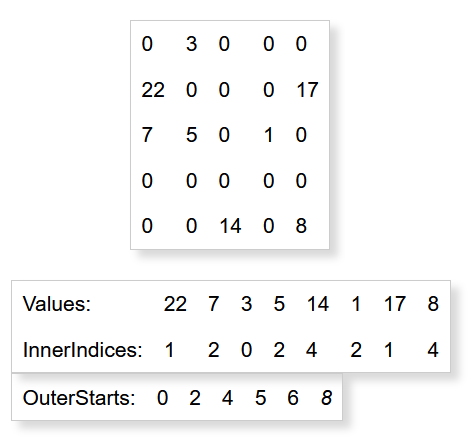
\includegraphics[width=0.35\textwidth]{spmat.PNG}
        \caption{A visual representation of a sparse matrix in the CSR format} \label{fig:sparse_matrix}
\end{figure}

I previously mentioned that multithreading Eigen would be a slightly wrong move. In my tests, Enabling Eigen's multithreading did not provide a significant speedup (or any at all). Some theories as to why this happened include: the fact that the matrix arithmetic operations exhibit false sharing (where two threads are writing to the same cache line, causing the cache to be invalidated and rewritten, which is a costly operation) or the overhead of creating threads being too large (implying that Eigen doesn't use a threadpool in its multithreading capabilities) \cite{kernel_false_sharing}. In the final implementation of this stage, I just disabled Eigen's multithreading capabilities and let the solver run on a single thread, since it proved to be just as good as the multithreaded version. Note that it could be possible for me to multithread the calculation across hinges/edges (assign each thread a set of hinges/edges to calculate the forces/Jacobians), but I did not pursue this optimization due to time constraints.

\subsection{Final Iteration of the DEP/S Algorithm: PARDISO Solver}
The final iteration of the DEP/S algorithm involved integrating the PARDISO solver from Panua Technologies \cite{Pasadakis2023} \cite{EFTEKHARI2021101389} \cite{gaedkemerzhäuser2022}. PARDISO is a direct solver that uses the parallel sparse LU factorization method to solve the matrix. In order to fully utilize PARDISO's potential, I had to change the underlying sparse matrix representation to only use the upper triangular part of the matrix, since the solver has optimizations for when the matrix is symmetric. This is implemented as a simple check before adding to the array of triplets (reject if col < row). Once the solver was integrated, the simulation experienced a 

\subsection{Rendering}
The rendering of the cloth is simple. The cloth is rendered as a mesh of triangles, with each edge outlined with red lines. The fixed nodes of the simulation are highlighted with cyan (and the viewer can clearly see their effect on the rest of the points). In the underlying implementation, to go around the issue of memory alignment(more on this later), I keep track of two arrays of positions: one for the cloth simulation and one for rendering. After the positions are calculated, I copy the positions from the simulation array to the rendering array, and then send the rendering array buffer to the GPU to be rendered. The use of two arrays was a lapse in judgement on my part that I will explain later. 


\section{Issues}
        I encountered numerous amounts of problems as I implemented the cloth simulation. Unlike problems I would like to answer with this project, these are issues that hindered my progress and/or still exist in the project. I will discuss the issues in the order that they were encountered.

\subsection{Renderer Design}
        As I was developing the cloth simulation, I realized that my renderer implementation was brittle, because it was coupled. The initial idea of my renderer design was that the client would first pass in a Scene object into a render call, then the renderer would call the OpenGL draw calls for each of the primitives in the scene. In OpenGL (which could be contextualized as an highly configurable state machine), one must supply state to the OpenGL context before a draw call is executed. The usual state for draws (which is bound to the context) includes the shader programs to be executed on the GPU, the vertex array objects specifying the format of the vertex data, the buffers containing the vertex data (the positions, the indices to those positions if using indexed rendering), and other buffers/data that the shaders need. The key point here is that the vertex array object had to be created for every known object type in my renderer because each new object had vertex data in different formats. Because I elected to have the renderer responsible for all drawing of the primitives, I stored all the vertex array objects for each type there. So if I had to add a new object type (like my cloth), I was forced to modify the renderer class as well. This directly goes against the idea of the Open-Closed Principle in software design. Some solutions to this include: using a visitor design pattern to render the objects, so that the renderer uses the common interface to render the objects, use a entity component system to separate the rendering logic from the object data, or use a factory pattern to create the vertex array objects for the objects and defining rendering logic for each object type.


\subsection{Subtlties in C++ and OpenGL}
        I was caught up in a few subtlties in the C++ language and OpenGL. For instance, I spent a huge amount of time relearning what C++ templates are. I derived my cloth system from a particle system interface because I wanted to allow the user to specify different parameters per system. Using templates opens the particle system to extension, so the user can customize the parameters and logic to supply to the system. The implementation of this (especially debugging) proved to be more arduious than I thought. Because templates were expanded upon instantiation of the object (it was a template that gets expanded into a class), the line that had the error of code was not indicated in the debug logs. This design also proved to be a less effective than perceived, supporting the idea that there are no zero cost abstractions \cite{caruth2019}. 

        Another subtlety I ran into was memory alignment issues in OpenGL. To start, the DEP algorithm assumes that the DOF vector is a $ 3 \times n $ by $ 1 $ column vector, where $n$ is the number of vertices. My initial naive implementation consisted of an array of 3 by n floats to represent the DOF vector used for calculating the forces and use the same DOF vector for drawing (specifying the vertex format to assume a vertex stream of vec3). This would work if I didn't use my DOF vector in the other (compute/debug) shaders (specifying the DOF vector as a shader buffer storage object (SSBO)).

        Before going further and to make things clear, I have a two shaders (programs run on a GPU): one shader used for the rendering of the cloth itself (cloth shader), another for highlighting the certain primitives such as edges, hinges, and fixed points (highlight shader). The cloth shader requires the DOF positions (containing the actual vertex data) to be passed in as a buffer. However, the highlight shader requires some method of retrieving points to be highlighted, whether it is through pasing the positions in directly or passing in an array of indices to the positions. I chose the latter because I was already updating the buffer for the cloth shader with new positions. Adding another buffer of positions would not only take up more space and be redundant, but also take marginally more compute time. I do acknowledge this assumes that indexing into a SSBO (shader storage buffer object) is faster than transfering the data from the CPU to GPU. Now because I elected to do the latter, I had to deal with memory alignment issues with my buffer. 

        However, according to the OpenGL specification, when using SSBOs and the std430 layout, a vec3 is aligned to 16 bytes (4 floats) in GPU memory. This means that in the shader, when I try to index into an array of vec3s, the GPU will retrieve the result with 3 floats plus 4 bytes of padding. So when I copy the chunk of buffer data (the DOF vector) from CPU memory into GPU memory, I had to ensure that the total memory size of the DOF buffer is a multiple of 16 bytes. Otherwise, the GPU would read 3 floats from the buffer, skip one float part of another point, and then read the next 3 floats, which is wrong. This means that after my force calculation, I had to create a way to send the data to the GPU such that my buffer acted as a vector of vec4s. This is still a naive answer however. 

        There is another solution to this issue without aligning the DOF vector to 16 bytes. Instead of having the GPU read the buffer as an array of vec4s/vec3s, I could pass the buffer to the GPU as an array of floats (avoiding the alignment issue entirely). Then the vertex stream for rendering for the shaders (specifically the highlight shader since the DOF positions must be read as a SSBO instead of a vertex stream) would be the indices of the particles themselves. Then in the shader, I could use the particle indices to compute the indices of the components of each DOF for that particle. 

        To add on to this, OpenGL actually allows the user to pass an array of doubles in as a vertex stream using \texttt{glVertexAttribLFormat} \cite{opengl_documentation} . This means I did not even need to cast the DOF vector from double to float before sending it to the GPU. The cast would still need to be done in the vertex shader since the vertex shader output for positions (\texttt{gl\_Position}) is specified as a float type. I unfortunately realized this too late, therefore it is not implemented. 

        Finally, I initially proposed to use OpenGL compute shaders to do the simulation on the GPU. The DEP algorithm (save for the matrix solve) is embarassingly parallelizable, so it would be a good candidate for a compute shader. However, OpenGL does not support matrix operations beyond 4 by 4 dimensions, which means I would need to implement this myself. The conjugate gradient solve is also a parallelizable operation, but this requires significant time to debug (and GPU debugging is much different than CPU debugging since there is no way to step through programs). I concluded that this is a huge undertaking, so I decided to stick with the CPU implementation.

\subsection{Eigen's implementation of sparse matrices}
        Although Eigen's sparse matrix modules yielded a massive speedup in the simulation, the steps to get there were astounding. The first issue I encountered was that Eigen sparse matrices do not support slicing. Slicing is the operation of taking a set of indices and using them to retrieve the respective rows and columns of a matrix to create a new submatrix. This is a common operation in Python Numpy, and it is supported by Eigen dense matrices too. But the sparse matrix API does not support this operation. Because I couldn't slice the final Jacobian matrix for the relevant free DOFs, I also couldn't blindly add triplets into the sparse entries to create that matrix. The sparse entries needed to be filled such that the final Jacobian matrix was the one directly used in the solver. 

        The solution comes to life when I made 2 observations. First, the values in the columns and rows of the Jacobian matrix (in the bending/stretching force calculations) corresponding to the fixed DOFs don't contribute to the Jacobian for free DOFs. Second, the only issue that needs attention when directly adding the values to the sparse entries for the Jacobian for free DOFs is the location(new row and column) of the values in the sparse matrix relative to the location of the original destination(old row and column). The new row and column is equal to the difference between the old row and column and how many fixed DOF rows and columns are before the old row and column. Although it is possible to calculate this new row and column at simulation time, it is much easier to just keep track of this old row/col to new row/col mapping in a separate array and index into it when adding the values to the sparse entries. 
        
        The second issue I encountered was that PARDISO does not use column major ordering for its sparse matrices. I originally set PARDISO to solve for a unsymmetric real matrix (which is wrong because the Jacobian is a symmetric matrix) and used column major ordering for that matrix (providing PARDISO with direct pointers to the underlying Eigen sparse matrix data). This didn't matter because the transpose of the symmetric matrix is the same as the matrix itself. However, when I changed the solver to solve for a symmetric real matrix (which only needed a upper triangular part of the matrix), I had to change the ordering of the calculation into row major ordering. This was a simple fix, but it was a huge headache to debug because the error messages from PARDISO were not helpful.

\subsection{Degeneracies}
        It is known that the DEP/S algorithm is prone to some degeneracies, such as when an edge collapses or when the altitude collapses \cite{Tamstorf2013discrete}. This may manifest int the calculation as a division by zero error during the solve, an infinite loop (the error never reaches the desired tolerance), or the cloth visually becomes a cloud of points (see figure \ref{"fig:chaos"}). These may arise when the solver is unable to reach a valid solution. This is more common in simulations with more DOFs as there is more freedom for numerical instability to occur. In my own tests, the most nodes I found that would reach the resting state without reaching numerical instability is 529 nodes (1575 DOFs, side length = 22). Of course, numerical instability could be mitigated by using a smaller timestep, but this would slow down the simulation (more time steps per second and more work to compute the next position at the next second). Another potential solution would be to check the solver solution before it updates the DOF vector. If the solution is degenerate, special care can be taken (i.e. halve the time step used for the rest of the iterations). Regardless, this problem requires more investigation to find a more robust solution.

\section{Remarks}
        The definition of real-time in this project is ill-posed. The simulation could be considered real-time, but only consist of 4 nodes (not exactly a cloth). The simulation could also be considered real-time if the timestep is large enough that the simulation is not accurate or stable. In the course of development, I kept trying to push the limits of the simulation to see how fast it could improve upon the first implementation. If the simulation was slower than it is now, I would have needed to define the question more concretely. 

        Accuracy and speed are always at odds with each other it seems. It is possible to get the simulation to run $n=22$ at 30 FPS if the error tolerance check was completely removed. Visually, there is no significant difference between that simulation and one with the error tolerance check, but the former is not accurate. The simulation is still confined by the nuance of numerical instability however (probably even more so). But now reducing the time step now has less of an effect on speed over all. This observation implies that the explicit integration method is worth looking into for future work.

        Finally, the DEP/S algorithm serves as a good basis for other material deforming features such as collision, viscous drag, tearing, friction, etc. Each of these could be implemented as an addition into the external forces or as a complete subroutine integrated into the internal force/jacobian calculation. Regardless, these features also take significant time to implement, debug, and compute (adding more work to a simulation that is already loaded). It may be rewarding to look into these feature in the future.


\section{Conclusion}

        In this report, I have presented the results of my cloth simulation project, detailed the process of implementing the DEP/S algorithm in C++ using the Eigen library and OpenGL and addressed the numerous issues I encountered during the implementation. The results proved that it is possible to run the DEP/S algorithm in real-time on a cloth with adequately high fidelity. In the future, I may look into optimizing the simulation further, adding more features to the simulation, and investigating solutions to mitigate degeneracies. But for now, I believe a refactoring of the renderer design is in order.  



\addtolength{\textheight}{-12cm}   % This command serves to balance the column lengths
                                  % on the last page of the document manually. It shortens
                                  % the textheight of the last page by a suitable amount.
                                  % This command does not take effect until the next page
                                  % so it should come on the page before the last. Make
                                  % sure that you do not shorten the textheight too much.

%%%%%%%%%%%%%%%%%%%%%%%%%%%%%%%%%%%%%%%%%%%%%%%%%%%%%%%%%%%%%%%%%%%%%%%%%%%%%%%%



%%%%%%%%%%%%%%%%%%%%%%%%%%%%%%%%%%%%%%%%%%%%%%%%%%%%%%%%%%%%%%%%%%%%%%%%%%%%%%%%

\bibliographystyle{ieeetr} % We choose the "plain" reference style
\bibliography{refs} % Entries are in the refs.bib file

\end{document}
